\documentclass[12pt]{article}
\usepackage{mathtools} 
\usepackage{amsthm,amssymb}
\usepackage{verbatim,comment,xcolor,graphicx,hyperref}
%\usepackage[papersize={4.5in, 6.2in}, width=4.13in, height=5.83in, vcentering, centering]{geometry} % Kindle-size pages
\usepackage[left=1.0in,right=1.0in,top=1.0in,bottom=1.0in]{geometry} % never use the anysize package!
\usepackage{mathpazo}

\newcommand{\degs}[1]{\textsuperscript{$\circ$}#1}
\definecolor{footlineblue}{rgb}{0.392,0.706,0.941}

\parskip=12pt
\parindent=0pt

% tikz stuff and other macros
% Jesse Hamner
% 2013--2017

% make a few color defs:
\definecolor{rltbrightred}{rgb}{1,0,0}
\definecolor{rltred}{rgb}{0.75,0,0}
\definecolor{rltdarkred}{rgb}{0.5,0,0}
\definecolor{rltbrightgreen}{rgb}{0,0.75,0}
\definecolor{rltgreen}{rgb}{0,0.5,0}
\definecolor{rltdarkgreen}{rgb}{0,0,0.25}
\definecolor{rltbrightblue}{rgb}{0,0,1}
\definecolor{rltblue}{rgb}{0,0,0.75}
\definecolor{rltdarkblue}{rgb}{0,0,0.5}
%\definecolor{webred}{rgb}{0.5,.25,0}
\definecolor{webblue}{rgb}{0,0,0.75}
\definecolor{webgreen}{rgb}{0,0.5,0}
\definecolor{lightgray}{gray}{0.9}
\definecolor{medgray}{gray}{0.6}
\definecolor{footlineblue}{rgb}{0.392,0.706,0.941}
\definecolor{darkgreen}{rgb}{0.00,0.50,0.00}
\definecolor{gray50}{gray}{0.50}
\definecolor{gray95}{gray}{0.95}
\definecolor{webred}{rgb}{0.75,0,0.0}

\renewcommand{\thefootnote}{\fnsymbol{footnote}}
\newcommand{\sep}{1mm}
\newcommand{\negsep}{-4mm}
\newcommand{\widesep}{7mm}
\newcommand{\thisscale}{0.6}

\newcommand{\+}{\item}		% easier than typing \item a lot
%\setlength{\parindent}{0in}	% easier than putting \noindent at every paragraph
\newcommand{\bi}{\begin{itemize}}
\newcommand{\ei}{\end{itemize}}
\newcommand{\bd}{\begin{description}}
\newcommand{\ed}{\end{description}}
\newcommand{\be}{\begin{enumerate}}
\newcommand{\ee}{\end{enumerate}}
\newcommand{\rr}{\raggedright}

\newcommand{\cb}{\cellcolor{black!35}}

\newcommand{\ckb}{\item[$\square$]} % list checkboxes (requires marvosym)

% A command that makes a uniform box around a paragraph. 
% It's a minipage environment, which means it doesn't support some commands.
\newcommand{\stbox}[2]{
	\begin{center}
	\fbox{
		\begin{minipage}[c]{#1}{
		\noindent #2
		}
		\end{minipage}
	}
	\end{center}
}


% A series of macros that enable programmatic of drawing stylized
% ions, protons, or electrons.
% Supports,  e.g., richer drawings of capacitors or
% current flowing in wires:

\newcommand{\ionradius}{0.06} % TODO should make it possible to change this too

\newcommand{\drawion}[4]{
		\draw [black, very thin] (#1,#2) circle [radius=#3];
		\node[scale=0.3, thick ] at (#1,#2) {#4};
}

\newcommand{\posion}[3]{
		\drawion{#1}{#2}{#3}{$+$}
		}

\newcommand{\negion}[3]{
		\drawion{#1}{#2}{#3}{$-$}
		}

\newcommand{\horizionarray}[4]{
	\newdimen\len
	\len=#1 cm
	\advance\len by -0.4cm
	\drawion{\len}{#2}{\ionradius}{#4}
	\advance\len by 0.15cm
	\drawion{\len}{#2}{\ionradius}{#4}
	\advance\len by 0.15cm
	\drawion{\len}{#2}{\ionradius}{#4}
	\advance\len by 0.2cm
	\drawion{\len}{#2}{\ionradius}{#4}
	\advance\len by 0.15cm
	\drawion{\len}{#2}{\ionradius}{#4}
	\advance\len by 0.15cm
	\drawion{\len}{#2}{\ionradius}{#4}
}

\newcommand{\vertionarray}[4]{
	\newdimen\len
	\len=#2 cm
	\advance\len by -0.4cm
	\drawion{#1}{\len}{\ionradius}{#4}
	\advance\len by 0.15cm
	\drawion{#1}{\len}{\ionradius}{#4}
	\advance\len by 0.15cm
	\drawion{#1}{\len}{\ionradius}{#4}
	\advance\len by 0.2cm
	\drawion{#1}{\len}{\ionradius}{#4}
	\advance\len by 0.15cm
	\drawion{#1}{\len}{\ionradius}{#4}
	\advance\len by 0.15cm
	\drawion{#1}{\len}{\ionradius}{#4}
}



% Nokia 84 x 48 pixel LCD screen (usually model number 5110 or 3310)
\newcommand{\drawnokiagrid}{
\draw[step=1cm,blue!30,very thin] (0,0) grid (6,8);
\foreach \x in {0,1,2,3,4,5}
	\draw (\x cm, 0pt) -- (\x cm, -3pt) node[anchor=north] {$\x$};
\foreach \y in {1,2,3,4,5,6,7,8}
	\draw (0pt, \y cm) -- (-3pt, \y cm) node[anchor=east] {$\y$};
}


% part of the Nokia grid set of commands
\newcommand{\msqo}[3]{
\def\mycmd{#3}

\if\mycmd1
	\msq{#1}{#2}{black!65}
\else
	\msq{#1}{#2}{white}
\fi
}


% part of the Nokia grid set of commands
\newcommand{\msq}[3]{
\edef\myx{#1}
\pgfmathparse{\myx+1.0}
\edef\myxtwo{\pgfmathresult}
\edef\myy{#2}
\pgfmathparse{\myy+1.0}
\edef\myytwo{\pgfmathresult}
\fill[#3] (\myx,#2) rectangle (\myxtwo,\myytwo);}


% part of the Nokia grid set of commands
\newcommand{\mcol}[9]{
\msqo{#1}{#2}{#3}
\msqo{#1}{#4}{#5}
\msqo{#1}{#6}{#7}
\msqo{#1}{#8}{#9}
}


% part of the Nokia grid set of commands
\newcommand{\hexlabel}[5]{
\node[rotate=90] at (0.5,-1) {\Large\texttt{#1}};
\node[rotate=90] at (1.5,-1) {\Large\texttt{#2}};
\node[rotate=90] at (2.5,-1) {\Large\texttt{#3}};
\node[rotate=90] at (3.5,-1) {\Large\texttt{#4}};
\node[rotate=90] at (4.5,-1) {\Large\texttt{#5}};
}



% drawing cubes using TikZ:
\newcommand{\makecube}[2]{
\begin{tikzpicture}[xscale=#2,yscale=#2]
\foreach \x in{0,...,#1}
{   \draw (0,\x ,#1) -- (#1,\x ,#1);
    \draw (\x ,0,#1) -- (\x ,#1,#1);
    \draw (#1,\x ,#1) -- (#1,\x ,0);
    \draw (\x ,#1,#1) -- (\x ,#1,0);
    \draw (#1,0,\x ) -- (#1,#1,\x );
    \draw (0,#1,\x ) -- (#1,#1,\x );
}
\end{tikzpicture}
}


% Draw faux-3D squares or cubes:
\newcommand{\makeplate}[3]{
\begin{tikzpicture}[xscale=#3,yscale=#3]

\foreach \x in {0,...,#1}
{
	\filldraw[gray95, fill=gray95, line width=0.0cm] (0,#1,0) -- (0,#1,#2) -- (#1,#1,#2) -- (#1,#1, 0) -- (0,#1,0) -- cycle;
	\filldraw[gray50, fill=gray50, line width=0.0cm] (#1,#1,0) -- (#1,#1,#2) -- (#1,0,#2) -- (#1,0, 0) -- (#1,#1,0) -- cycle;
}

\foreach \x in{0,...,#1}
{   \draw (0,\x ,#2) -- (#1,\x ,#2);
    \draw (\x ,0,#2) -- (\x ,#1,#2);
	\draw (#1,\x ,#2 ) -- (#1,\x ,0);
    \draw (\x ,#1,#2 ) -- (\x ,#1,0);
}

\foreach \x in {0,...,#2}
{
    \draw(#1,0,\x  ) -- (#1,#1,\x );
    \draw(0,#1,\x  ) -- (#1,#1,\x );
}

\foreach \x in{1,...,#1}
{
\node[align=left] at (\x-0.5,#1-0.5,#2) {\x};
}

\foreach \x in{#1,...,2}
{
\node[align=left] at (0.5,#1-\x+0.5,#2) {\x};
}

%\draw[webred, thick](0,0,0) -- (0,0,#2);
%\draw[webblue, thick](0,0,0) -- (#1,0,0);
%\draw[darkgreen, thick](0,0,0) -- (0,#1,0);

\end{tikzpicture}
}


% Draw a line of faux-3D shaded blocks using TikZ:
\newcommand{\blockline}[2]{
\begin{tikzpicture}[xscale=#2,yscale=#2]

\filldraw[fill=gray95, ultra thin] (0,1,0) -- (0,1,1) -- (#1,1,1) -- (#1,1, 0) -- (0,1,0) -- cycle;
\filldraw[fill=gray50, ultra thin] (#1,1,0) -- (#1,1,1) -- (#1,0,1) -- (#1,0, 0) -- (#1,1,0) -- cycle;

\draw (0,1,0 ) -- (#1,1,0); % top line
\draw (#1,1,1) -- (#1,1,0);
\draw (#1,0,1) -- (#1,1,1);
\draw (0,1, 1) -- (#1,1,1);
\draw (0,0,1 ) -- (#1,0,1);

\foreach \x in{0,...,#1}
{   
    \draw (\x ,0,1) -- (\x ,1,1 ); % straight vertical lines    
    \draw (\x ,1,1) -- (\x ,1,0 );
}

\foreach \x in{1,...,#1}
{
	\node[align=left] at (\x-0.5,0.5,1) {\x};
}

\end{tikzpicture}
}


% make a blank line under which, e.g., someone could write an unknown answer:
\newcommand{\makeblank}[1]{
\underline{\makebox[#1][l]{}}
}


% tilt the text atop a table row at an angle:
\newcommand*\rot{\multicolumn{1}{R{55}{1.2ex}}}% no optional argument here, please!

\graphicspath{{../images/}}

\begin{document}

\thispagestyle{empty}
\date{}
\title{Soldering Tutorial}
\author{Jesse Hamner}


\maketitle

\begin{abstract}
Learning to solder opens up a broad and deep section of STEM and STEAM education. Children, when equipped with tools that allow them greater access to electronic devices, tools, and programming, will get an early understanding of how electricity works, and how electronics are made. This tutorial, originally written for undergraduate-level novices, is a 2-hour workshop taking children from the most basic ideas of soldering, through a completed, if simple, soldering project.\\
~\\
\textbf{Keywords:} STEM; education; electronics; elementary education; soldering.

\end{abstract}

\begin{center}
\fbox{
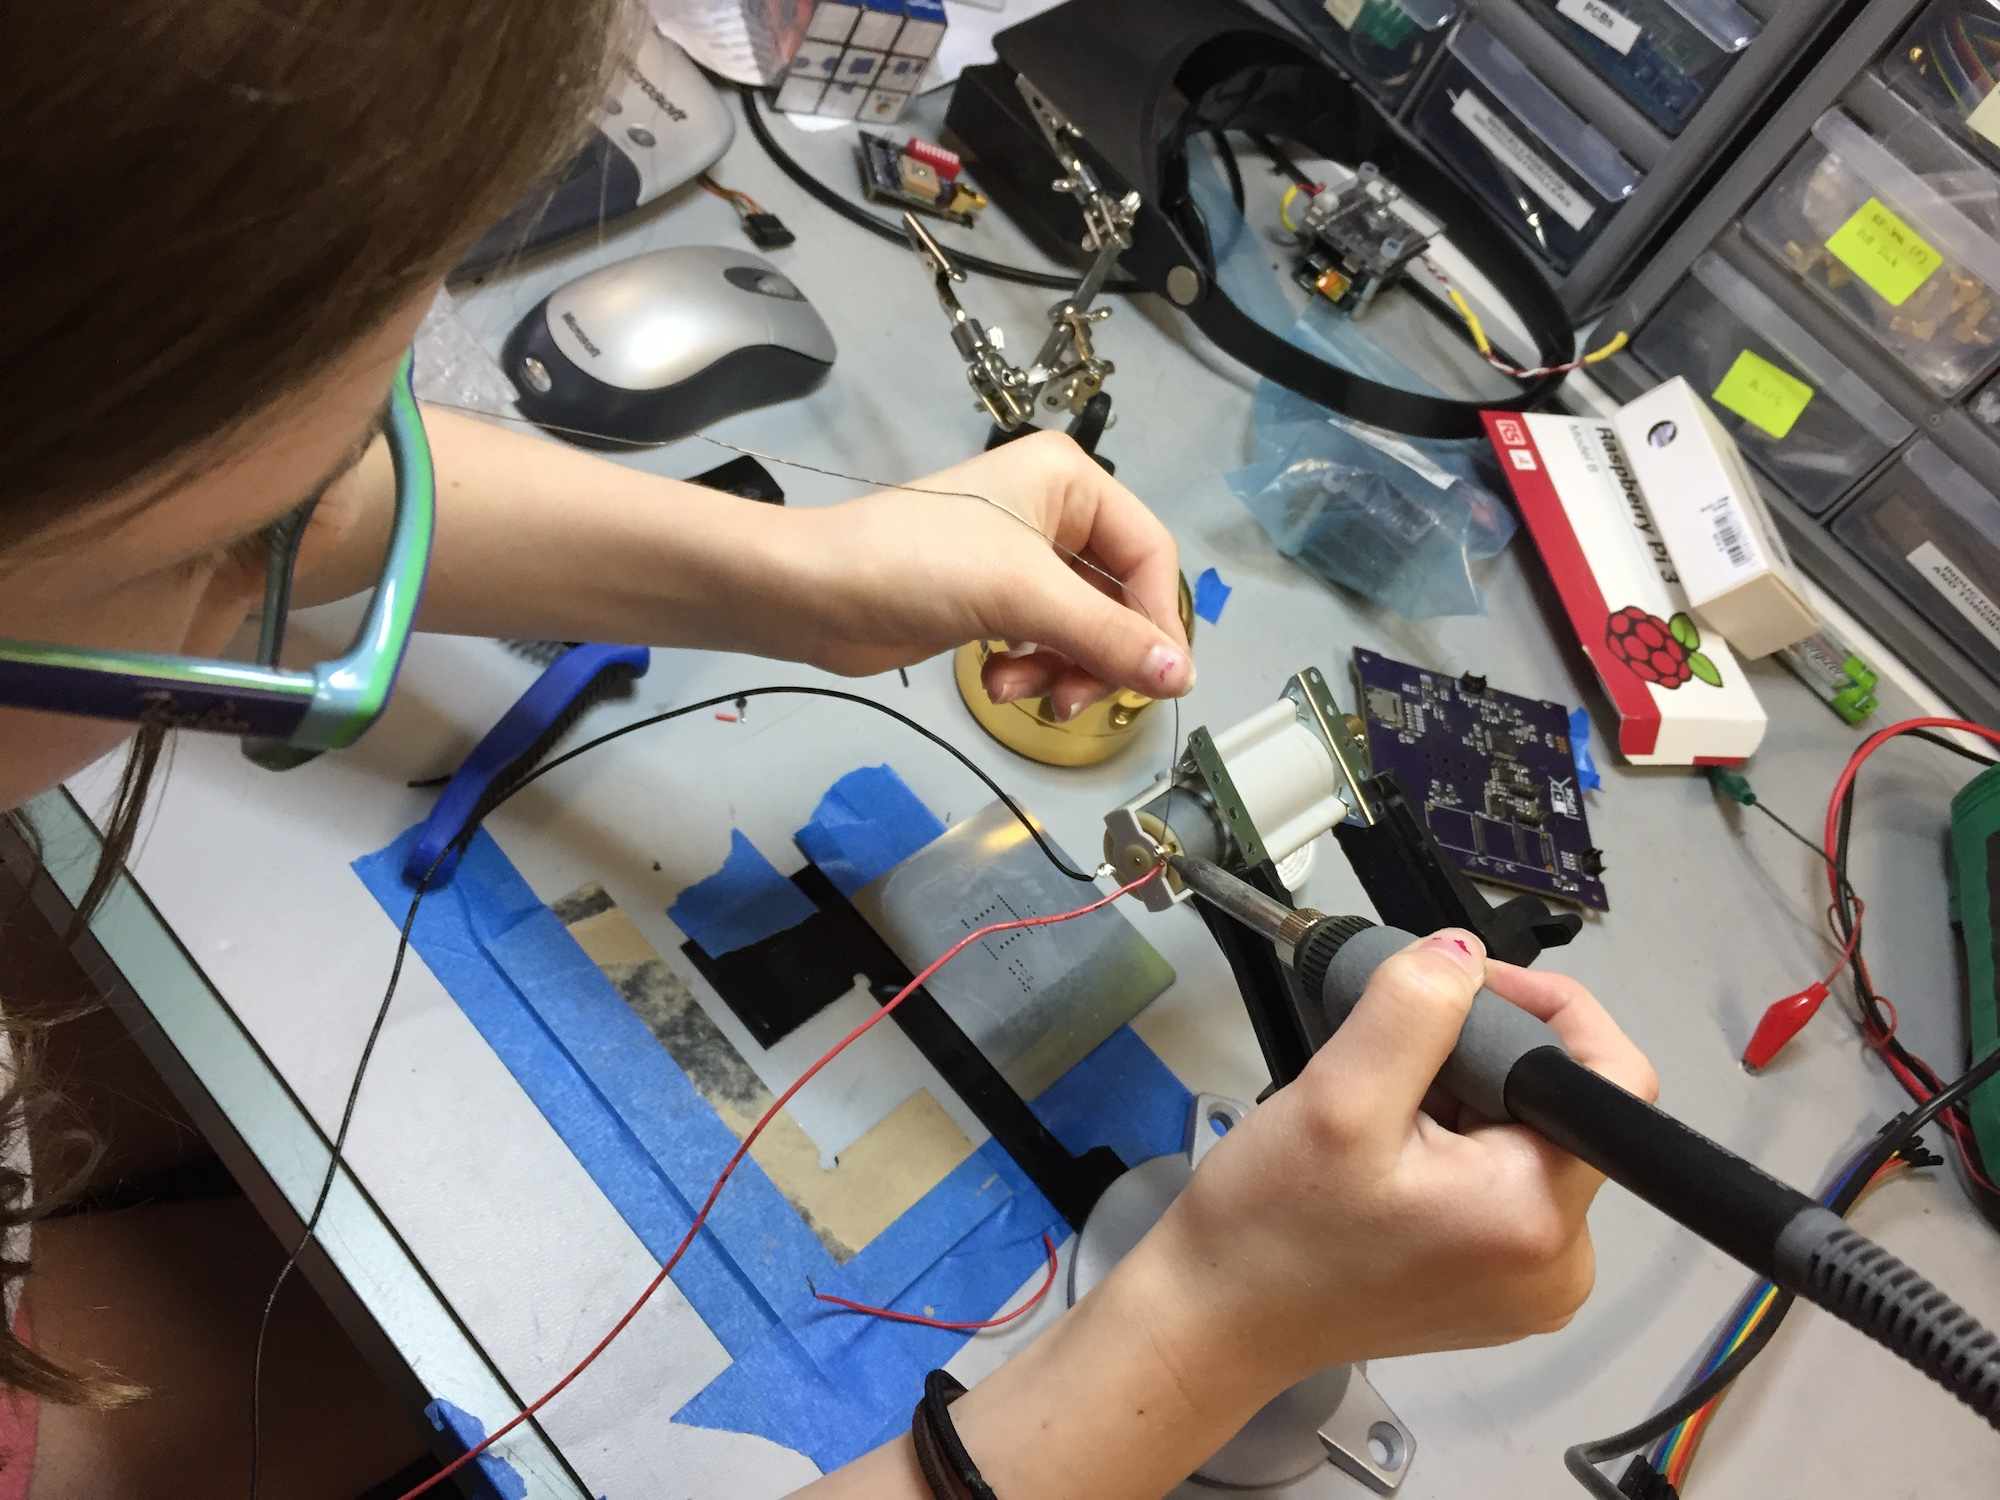
\includegraphics[scale=0.14]{soldering.jpg}
}

The author's daughter, repairing a DC motor for her elementary school.
\end{center}

\vfill

\begin{center}
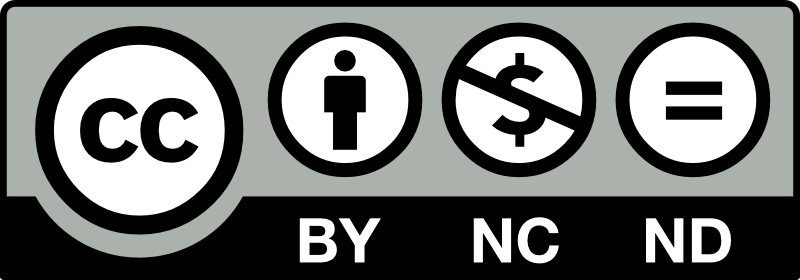
\includegraphics[scale=1.0]{by-nc-nd.png}

This work is licensed under a {\color{webblue}\href{https://creativecommons.org/licenses/by-nc-sa/4.0/}{Creative Commons Attribution-NonCommercial-ShareAlike 4.0 International License.}} 
% Attribution-NonCommercial-ShareAlike 4.0 International (CC BY-NC-SA 4.0)
\end{center}


\newpage
\section{Vocabulary}

\begin{description}

\+[Soldering:] The use of molten metals to electrically and physically bond other metals together, such as pipe, wire, or electronic components.

\+[Tin:] Metal common to virtually all solder compositions. More expensive than lead, but makes it easy to ``wet'' the metals being joined. Melting point: 450\degs{F}/232\degs{C}

\+[Lead:] Obviously poisonous, but does not produce fumes at soldering temperatures. Up to about 40\% of some solder compositions. Inexpensive. Melting point: 621\degs{F}/327\degs{C} Almost all of the electronics industry has moved to no-lead components and solder, but lead makes for a very forgiving solder. The amount of lead to which you will be exposed is very small, and provided you wash your hands after handling it, will not affect you at all.

\+[Silver:] An exceptional thermal and electrical conductor; has the lowest resistance by 30\% (gold being the runner-up)  among pure elements. Notable also because even silver oxide is an excellent conductor. Makes up a small proportion of no-lead solders, usually around 4\%. Very expensive. Melting points range from 880--960\degs{C} (1615/1760\degs{F}). 

\+[Copper:] Moderately expensive metal. Used in no-lead solder in small amounts. Melting point 1084\degs{C}/1983\degs{F}. 

\+[60/40 solder:] Along with 63/37 solder, the most common lead solder composition. 63/37 has the lowest melting point of all tin/lead solders, at 361\degs{F}/183\degs{C}. 60/40 melts at 188\degs{C}/370\degs{F}. 

\+[Lead-free solder:] Typically tin-silver-copper, with a melting point 10\degs{C} or so higher than common lead solders. More difficult to unsolder. Expensive. Almost all tin (well over 90\%).

\+[Flux:] from the Latin meaning ``to flow", flux cleans metallic surfaces of oxides (usually with some kind of acid), prevents oxides from forming, and reduces the surface tension of molten solder (put another way, it improves ``wetting'' of metals with the molten solder). Oxides usually resist solder bonding, and oxides form quickly at high temperatures. Flux is really important. Most solder now has a supply of flux contained in the solder wire itself, but there are flux pens for cases where you need more flux, like surface-mount soldering and component de-soldering.

\+[Eutectic:] a metal alloy having a lower melting point than any of its component metals. Weird, right? Solder is a eutectic alloy, and that's very useful for soldering---it can bind wires or components together without melting the metal (melting metals together is \emph{welding}).

\+[Gauge:] the thickness of a wire according to a very old American standard system. It is more convenient to ask for ``20-gauge solder'' than to say ``0.032-inch'' or ``0.8 millimeter'' thickness.

\+[Through-hole:] The earliest and simplest means to attach individual electronic components to a printed circuit board: holes in the board have metal linings, and \emph{traces} of copper from the board make up the electrical connections between components, instead of loose/discrete wires. Soldering through-hole components is really easy and looks professional.

\+[Surface-mount technology (SMT):] The modern, high-density, means to attach components to circuit boards. No holes -- instead, tiny solder blobs hold the small (usually very small!) components to one side of the board, and don't require holes. Additionally, they don't make a hole in the other side of the board that traces have to route around. SMT soldering is a quite different skill from through-hole soldering, but the results are usually impressive, efficient, and cheaper than through-hole designs. But not for beginners.

\+[Dual In-line Package (DIP):] the oldest form factor for integrated circuits (chips). Pins are spaced 0.1" apart. Rows are usually 0.3" or 0.6" apart, and the pins can be through-hole soldered or put into sockets. A DIP is usually referred to as a DIP\emph{n}, where \emph{n} is the total number of pins, with each row having half the overall count of pins. 

\+[Surface-mount packages:] chips where the pins do not go through the board, even if the pins are 0.1" apart or built on a DIP carrier. The pins on these chips get too small to reliably solder with a soldering iron, but plenty of surface-mount parts can be reliably soldered with a regular iron.

\+[Soldering iron:] a pencil-shaped tool with a removable tip (tips come in various shapes) that gets hot enough to melt solder. Usually powered by electricity, but some use butane heaters.

\+[Soldering iron tips:] varying shapes of the hot end of the soldering iron are suited for general or special purposes. The most common is the \emph{chisel} tip, although these come in varying widths. \emph{Hoof} tips are adapted for soldering surface-mount chips. \emph{Conical} tips appear to be very precise, as they concentrate all the heat into a very small point, but that point is usually insufficiently large to transfer enough heat to all but the smallest components---ones you're unlikely to be working with.

\+[Solder sucker:] a small, spring-loaded vacuum pump, allowing the user to heat a defective or wrongly-placed solder joint, and pull almost all the solder away from the joint. The joint can then be separated without pliers or damage.

\+[Solder braid:] A flat, woven cable of loose copper fibers, usually covered in solid flux. Copper transfers heat rapidly, and capillary action of the tiny fibers makes it possible to remove solder from a joint without a solder sucker. A higher difficulty of use, but produces good results.

\+[Thermal shock:] damage to components caused by physical strain on a component that is heated or cooled too rapidly (different points expand differently, depending on how hot or cold they get over some small slice of time).

\+[Thermal damage:] overheating a component, impairing its function or destroying it completely. See also: ``letting out the magic smoke.''

\+[Thermal tolerance:] how much heat (what temperature and for how long) a given component can handle before damage occurs. These specifications are always provided in the data/specs sheets.

\+[Cold Solder Joint:] It is possible to put solder on a joint and not electrically connect the metallic components. Hugely frustrating to diagnose -- the joint usually appears to be complete. Always caused by insufficient heating of the solder joint. 

\+[Hot air rework:] Using a stream of super-heated air to heat a solder joint instead of direct contact with a metal tip. Typically slower, and runs a greater risk of thermal damage to a component. But for desoldering work, it's usually a great choice.

\+[Solder paste:] ``spreadable" solder with flux and solder in a paste, instead of a wire. When combined with hot air rework, or a reflow oven, solder paste allows you to solder all the components you want to solder at once. Thus you expose all items to heat at once -- and all the soldering happens simultaneously.

\+[Ohm:] Abbreviated $\Omega$, an Ohm is a unit of resistance to electrical flow. One Ohm is a very small amount of resistance. 10,000 Ohms (10K$\Omega$) is a moderate amount of resistance. 10 megaohms (10M$\Omega$) is a lot of resistance. Resistors dissipate some electricity as heat. The greater the resistance for a given voltage, the lower the current will be. This is Ohm's Law: $V=IR$ 

I is current, R is resistance, and V is voltage.

\end{description}

\begin{center}
\fbox{

\includegraphics[scale=0.55]{bobpease.png}
}
\end{center}

\newpage

\section{Bill of Materials}

For this exercise, we need:
\begin{enumerate}
\+ wire strippers
\+ pliers
\+ soldering iron
\+ wire solder (leaded or no-lead)
\+ diagonal cutters or flush cutters
\+ solder sucker
\+ masking tape
\+ third hand and/or Panavise
\+ brass cleaner sponge
\+ flush cutters (optional)
\+ some quantity of small-gauge insulated electrical wire (solid or stranded, but solid is better for this tutorial)
\+ three through-hole, $\frac{1}{4}$ watt resistors per person (10K$\Omega$, 1K$\Omega$, and 220$\Omega$)
\+ one through-hole, leaded LED per person
\+ one simple soldering kit:
	\begin{itemize} 
	\+ Sparkfun's {\color{webblue}\href{https://www.sparkfun.com/products/10723}{WeevilEye}}, \$10, is a great choice
	\+ Maker Shed's {\color{webblue}\href{http://www.makershed.com/products/learn-to-solder-skill-badge-kit}{Makey Robot Badge}}, \$3, is another
	\+ logic gate PCBs (designed by the author and suitable for beginners, though some of the parts do get close together)
	\end{itemize}
\+ shrink tubing (optional)
\end{enumerate}


\newpage
\section{Tutorial}

\subsection{Setup}

Everyone should have:

\begin{enumerate}
\+ A beginner-level soldering kit, like the WeevilEye
\+ Three through-hole, 1/4 watt resistors (10K$\Omega$, 1K$\Omega$, and 220$\Omega$)
\+ One through-hole, leaded LED
\+ Three 4-inch pieces of small-gauge wire
\+ A place to work while seated
\+ Access to the hand tools and soldering tools
\end{enumerate}

Next:

Get a soldering iron. Ensure the end of the iron is safely in its holder. Power up the iron. Ensure the temperature is set to about 650\degs{F} or 700\degs{F}.  Set up the third hand, if you have one. Strip about $\frac{1}{4}$\textsuperscript{\texttt{"}} off of two pieces of wire and discard the insulation.

\subsection{Flux and Solder}

When the temperature reaches the set point, touch a bit of solder to the tip. The smoke is flux, not lead! You now have a blob of no-flux solder on the end of your soldering iron. Hook the piece of wire to a third hand or a pair of pliers. Touch the solder blob to the piece of stripped wire. Try to get the solder off onto the wire. Leave the tip and solder in contact with the wire, then touch a bit more solder to the joint. The solder will run right onto the wire. Clean excess solder from the tip of the soldering iron with a brass sponge.

\subsection{Solder two wires}

Strip the other end of the wire. Strip both ends off of another piece of wire, producing at least $\frac{3}{8}$ inch of bare wire. Twist the wires together with pliers or fingers. Hold both wires in a pair of pliers or with a third hand. Heat the wire joint with the soldering iron. Keep the tip in contact with the joint you're soldering the whole time you want to apply solder. Touch solder to the hot twisted wires (\emph{not the soldering tip!}). You won't have to wait more than a second for the solder to melt, smoke, and run all over the joint. You won't need to use more than $\frac{1}{8}$ or $\frac{1}{4}$ inch of solder to completely cover the joint. Remove the solder. Carefully remove the iron tip immediately afterwards. The joint will cool quickly, but the wires may still be hot. Wait 15 seconds or so and check the temperature. Don't ever apply water to a hot solder joint or immerse the joint in water to cool it down. This will usually cause thermal shock and either separate the joint or make it very weak.

\subsection{Solder two resistors}

Let's make a voltage divider! The joint between two resistors (with power on one side and ground on the other) will have a voltage proportional to the input voltage, equivalent to

\begin{Large}
\begin{equation*}
V_{out} = V_{in} \times \frac{R_2}{R_1 + R_2}
\end{equation*}
\end{Large}

For a bit of extra skill development, solder a wire to the center leads. You'll need to decide if you can wrap it effectively and solder it, or if you need to get creative. Huge solder joints are unsightly, wasteful, and potentially harmful, so work carefully.

\subsection{Solder a resistor to an LED}

LEDs are just diodes that make light. They have very little resistance to current flow, meaning you can burn out a diode (\emph{any} diode, including LEDs) if you don't limit the amount of current flowing through it towards ground. Some LEDs have built-in subminiature current-limiting resistors, but never assume they do. LEDs are useful diagnostic tools, in the absence of anything else; you can see whether a section of a circuit is receiving power or not. This is a silly tool to make, but you're learning to solder right now, so play along. Find the short lead on the LED: this is the negative (cathode) pole. This end goes towards ground. Twist this lead and one end of the 220$\Omega$ resistor together. Solder them. 

\subsection{Solder a kit}

Now you are probably good enough to solder a simple through-hole kit. Your challenge, then, for this project is \emph{gravity}. Soldering components to the board really can't be done from the ``top'' side, unless you're using surface mount components. Thus, you have to keep the components in place while you flip the board over and solder the ``underside.'' There are two common ways to achieve this, not including the uncomfortable and dangerous ``hold it in place with your finger.'' First, you can bend the leads of the component away from each other, ensuring that the component can't fall out when you invert the board. Second, you can use masking tape to tape the component in place. It's much slower to tape something in place, but it's predictable and safe.

Once you solder a component in place, clipping the leads is required. Clip the leads with a wire cutter, flush cutter, or diagonal cutters. It is fine to clip the leads completely flush with the board, though the joints are a little stronger if you leave even half a millimeter or so of wire poking through. 

Once you complete the kit, and before you apply power, it's a good idea to check your connections with a continuity tester (of course, remembering that capacitors look like broken circuits to direct current and thus won't be ``continuous''\footnote{Capacitors can transfer alternating current, though they delay the signal by one quarter wave ($90^{\circ}$), potentially pushing the signal out of phase.}). But for something so simple, and safe, as this kit, you can probably be forgiven for applying power right away.

\section{Advanced topics}

Not really suitable for smaller kids, but something to at least tell the students about, so that they know there's more to do.

\begin{enumerate}
\+ soldering components in tight spaces
\+ soldering SMT components (you'd be surprised how small you can competently solder!)
\+ soldering with microscopes
\+ SMT integrated circuit packages
	\begin{itemize}
	\+ flux pens
	\+ tacking ICs into place
	\+ drag soldering across fine-pitch pins
	\+ the miracles of capillary action
	\end{itemize}
\+ solder paste
\+ hot air rework
\+ solder stencils, reflow ovens and skillets
\end{enumerate}

\end{document}
